\documentclass[a4paper, 12pt]{article}
\usepackage[utf8]{inputenc}
\usepackage[T1]{fontenc}
\usepackage[ngerman]{babel}
\usepackage{geometry}
\usepackage{listings}
\usepackage{xcolor}
\usepackage{hyperref}
\usepackage{helvet}
\usepackage{titlesec}
\usepackage{setspace}
\usepackage{graphicx}
\usepackage{pdfpages}
\usepackage{fancyhdr}
\usepackage{float}
\usepackage{enumitem}
\usepackage{tikz}
\usepackage{etoolbox}
\usepackage{tabularx}
\usepackage[style=apa, backend=biber, date=iso8601, urldate=iso8601]{biblatex}

%\addbibresource{bibs/citavi.bib}

%\DeclareFieldFormat{urldate}{
%    Abgerufen am \thefield{urlday}\adddot\addspace\mkbibmonth{\thefield{urlmonth}}\addspace\thefield{urlyear} von
%}

\hypersetup{breaklinks=true}

\definecolor{green}{HTML}{34A853}
\definecolor{orange}{HTML}{FBBC05}
\definecolor{red}{HTML}{EA4335}

\lstdefinelanguage{JavaScript}{
    keywords={break, case, catch, continue, debugger, default, delete, do, else, finally, for, function, if, in, instanceof, new, return, switch, this, throw, try, typeof, var, void, while, with},
    keywordstyle=\color{blue}\bfseries,
    ndkeywords={class, const, enum, export, extends, import, super, implements, interface, let, package, private, protected, public, static, yield, null, true, false},
    ndkeywordstyle=\color{darkgray}\bfseries,
    identifierstyle=\color{black},
    sensitive=false,
    comment=[l]{//},
    morecomment=[s]{/*}{*/},
    commentstyle=\color{purple}\ttfamily,
    stringstyle=\color{red}\ttfamily,
    morestring=[b]',
    morestring=[b]"
}

\lstset{
    language=JavaScript,
    extendedchars=true,
    basicstyle=\footnotesize\ttfamily,
    showstringspaces=false,
    showspaces=false,
    numbers=left,
    numberstyle=\footnotesize,
    numbersep=9pt,
    tabsize=2,
    breaklines=true,
    showtabs=false,
    captionpos=b
}
\geometry{a4paper, left=2.5cm, right=2.5cm, top=3cm, bottom=3cm, headsep=1.5cm}

\setlength{\parindent}{0pt}
\setlength{\parskip}{6pt}
\graphicspath{ {./images/} }

\pagestyle{fancy}
\fancyhf{}
\rhead{\vspace{0.2cm}
\includegraphics[width=4cm]{hs_mainz_logo}}
\fancypagestyle{plain}{
    \fancyhf{}
    \rhead{\vspace{0.2cm}
\includegraphics[width=4cm]{hs_mainz_logo}}
}
\renewcommand{\headrulewidth}{0pt}
\renewcommand{\footrulewidth}{0pt}
\fancyfoot[C]{\thepage}

\newcounter{lastroman}
\newrobustcmd{\switchtopage}[1]{
    \clearpage
    \setcounter{lastroman}{\value{page}}
    \pagenumbering{#1}
}
\newrobustcmd{\switchback}{
    \clearpage
    \pagenumbering{Roman}
    \setcounter{page}{\value{lastroman}}
}

% Document
\begin{document}

    \pagenumbering{Roman}

    \begin{titlepage}
    \centering
    \vspace*{1cm}

    
\includegraphics[width=0.4\textwidth]{hs_mainz_logo}\\
    \vspace{1.5cm}

    \textbf{\LARGE Praxismodul III}\\
    \vspace{0.5cm}
    \textbf{\Large Collectiqo}\\
    \vspace{1.5cm}

    \textbf{Hochschule Mainz}\\
    \vspace{0.5cm}
    Fachbereich Wirtschaft\\
    \vspace{0.5cm}
    B.Sc. Wirtschaftsinformatik dual\\
    \vspace{1.5cm}

    \textbf{Autoren:}\\
    Bindernagel, Lorenz\\
    Schäfer, Robin\\
    Šimić, Darko\\
    Struve, Anika\\

    \vspace{1.5cm}
    
    
\includegraphics[width=0.4\textwidth]{collecta-as-logo}\\
    \vfill

    \today
\end{titlepage}
    \newpage

    \textbf{Nützliche Informationen:}\par
\vspace{0.5cm}
GitHub Repository:\par
\url{https://github.com/LorackDev/collectiqo}\par
Datei für die Umgebungsvariablen ist nicht im Repository hinterlegt!\par
Die Docker Compose Datei befindet sich auf der obersten Ebene des Repositories.\par

\vspace{0.5cm}
Dockerhub Hauptapplikation:\par
\url{https://hub.docker.com/repository/docker/lorackdev/clq-node-multiarch/general}\par
Dockerhub Custom MySQL:\par
\url{https://hub.docker.com/repository/docker/lorackdev/clq-mysql-multiarch/general}\par
Dockerhub Custom MongoDB:\par
\url{https://hub.docker.com/repository/docker/lorackdev/clq-mongodb/general}\par

\vspace{0.5cm}
Aufruf der Applikation über den vServer:\par
\url{https://www.collectiqo.com}\par
    \newpage

    \setcounter{page}{2}
    \tableofcontents
    \newpage

    \switchtopage{arabic}

    \section{Projektplanung- und Management}\label{sec:section-one}

Lorenz ipsum dolor sit amet, consetetur sadipscing elitr, sed diam nonumy eirmod tempor invidunt ut labore et dolore magna aliquyam erat, sed diam voluptua.
At vero eos et accusam et justo duo dolores et ea rebum.
Stet clita kasd gubergren, no sea takimata sanctus est Lorenz ipsum dolor sit amet.

\subsection{Rückblick auf Praxismodul I \& 2}\label{subsec:subsection-one-one}

Lorenz ipsum dolor sit amet, consetetur sadipscing elitr, sed diam nonumy eirmod tempor invidunt ut labore et dolore magna aliquyam erat, sed diam voluptua.
At vero eos et accusam et justo duo dolores et ea rebum.
Stet clita kasd gubergren, no sea takimata sanctus est Lorenz ipsum dolor sit amet.

\newpage

\subsection{Zielsetzungen im Praxismodul III}\label{subsec:subsection-one-two}

Lorenz ipsum dolor sit amet, consetetur sadipscing elitr, sed diam nonumy eirmod tempor invidunt ut labore et dolore magna aliquyam erat, sed diam voluptua.
At vero eos et accusam et justo duo dolores et ea rebum.
Stet clita kasd gubergren, no sea takimata sanctus est Lorenz ipsum dolor sit amet.


\subsection{Projektorganisationen}\label{subsec:subsection-one-three}

Lorenz ipsum dolor sit amet, consetetur sadipscing elitr, sed diam nonumy eirmod tempor invidunt ut labore et dolore magna aliquyam erat, sed diam voluptua.
At vero eos et accusam et justo duo dolores et ea rebum.
Stet clita kasd gubergren, no sea takimata sanctus est Lorenz ipsum dolor sit amet.

\subsection{Verwendete Tools}\label{subsec:subsection-one-four}

Lorenz ipsum dolor sit amet, consetetur sadipscing elitr, sed diam nonumy eirmod tempor invidunt ut labore et dolore magna aliquyam erat, sed diam voluptua.
At vero eos et accusam et justo duo dolores et ea rebum.
Stet clita kasd gubergren, no sea takimata sanctus est Lorenz ipsum dolor sit amet.

\begin{figure}[H]
    \centering
    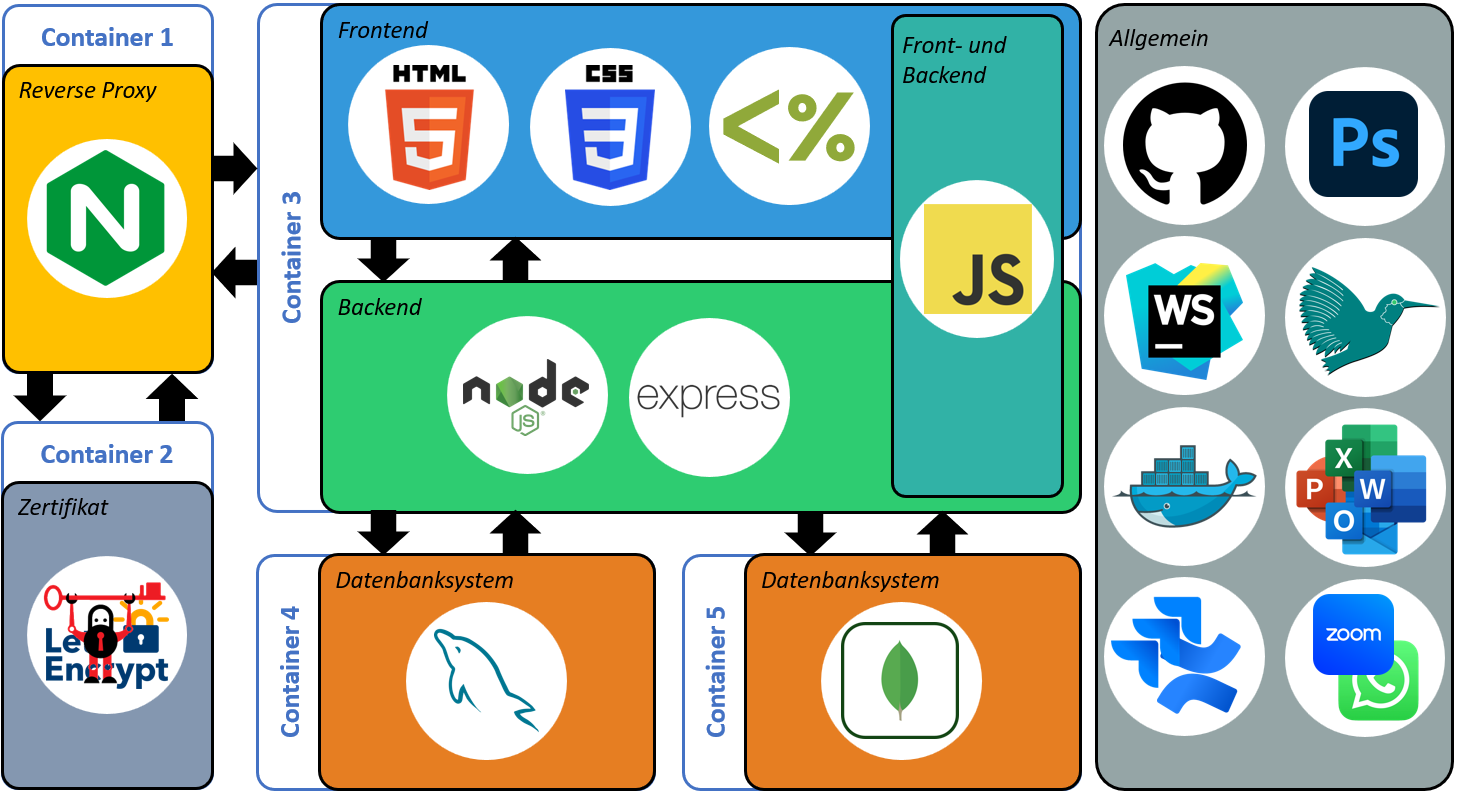
\includegraphics[width=1.0\textwidth]{tools}
    \caption{Übersicht der Tools}\label{fig:uebersicht-tools}
\end{figure}

\subsection{Arbeit mit Pull Requests und Restrictions in Git}\label{subsec:arbeit-mit-pull-requests-und-restrictions-in-git}

Im aktuellen Praxismodul III wurde die bereits im vorherigen Semester eingeführte Arbeitsweise mit separaten Feature-Branches weiterentwickelt und professionalisiert.
Während die Nutzung von Branches bereits in Praxismodul II etabliert wurde, lag der Fokus nun darauf, den Entwicklungsprozess durch verbindliche Strukturen und Regeln qualitativ weiter zu verbessern.

Neu eingeführt wurden sogenannte Pull Requests (PRs), über die Änderungen aus einem Feature-Branch nicht mehr direkt, sondern nur nach expliziter Prüfung durch ein Review in den `main`-Branch übernommen werden dürfen.
Dazu wurden feste Reviewer pro Pull Request definiert, die jeweils für die Freigabe verantwortlich sind.
Bei größeren Änderungen wurde gemeinsame Review Sitzungen während Team Meetings durchgeführt.
Zusätzlich wurden Git-Restrictions aktiviert, welche das direkte Pushen in den `main`-Branch unterbinden.
Dadurch ist sichergestellt, dass keine unkontrollierten Änderungen in die stabile Hauptversion gelangen.

Diese Weiterentwicklung der Git-Nutzung brachte folgende Vorteile mit sich:
\begin{itemize}
    \item Durch Reviews und Restrictions wurden potenziell fehlerhafte oder ungetestete Änderungen frühzeitig erkannt.
    \item Gemeinsame Review Sessions haben zu umfangreicherem Wissenstransfer innerhalb des Teams gesorgt.
    \item Die stabile Version im `main`-Branch konnte nicht durch versehen und unsauberes Arbeiten überschrieben werden.
\end{itemize}

Gleichzeitig entstanden aber auch folgende Herausforderungen:
\begin{itemize}
    \item Im Team musste vorerst ein Verständnis über den neuen Workflow geschaffen werden.
    \item Auch für kleinere Änderungen waren nun zusätzliche Review-Schritte notwendig.
\end{itemize}

Allgemein hat die Einführung der neuen Herangehensweise zu einer strukturierten Arbeitsweise geführt.

    \newpage

    \section{Visuelles Redesign}
    \newpage
    
    \input{sections/04-überarbeitung-der-sammlungserstellung}
    \newpage

    \section{Ausbau der Nutzereinstellungen}\label{sec:ausbau-der-nutzereinstellungen}

In diesem Kapitel wird die Erweiterung der Nutzereinstellungen beschrieben.
Ziel war es, Nutzern mehr Kontrolle über ihr Konto zu geben, insbesondere im Hinblick auf die Verwaltung von Zugangsdaten und Authentifizierungsinformationen.
Aufbauend auf dem bestehenden Frontend wurde das Backend um verschiedene Funktionalitäten ergänzt, welche die Selbstverwaltung der Nutzerkonten ermöglichen.

\subsection{Frontend}\label{subsec:frontend}

\subsection{Backend}\label{subsec:backend}

Im Rahmen des dritten Praxismoduls wurde das Backend zur Verwaltung von Nutzereinstellungen weiterentwickelt.
Aufbauend auf dem Frontend aus dem vorherigen Semester wurde die serverseitige Logik ergänzt, um Änderungen an Benutzerdaten sicher zu verarbeiten.
Die umgesetzten Funktionen umfassen die Änderung von Benutzername, Passwort und E-Mail-Adresse sowie das Ausloggen eines Nutzers.
Zur Datenverarbeitung wird eine Kombination aus MySQL (für Nutzerdaten) und MongoDB (für sammlungsbezogene Informationen) verwendet.
Die Implementierung folgt dem etablierten Aufbau aus Route, Controller und Service.
Da die Aufteilung bereits in der Dokumentation des Praxismoduls II erklärt wurde, wird hier nicht näher darauf eingegangen.

\subsubsection{Ändern des Benutzernamens}\label{subsubsec:username-update}

Die Funktion zur Änderung des Benutzernamens prüft zunächst, ob der alte Benutzername existiert und ob der neue Benutzername bereits vergeben ist.
Anschließend wird der Name sowohl in der MySQL-Datenbank als auch in den relevanten MongoDB-Collections aktualisiert:

\begin{lstlisting}[language=JavaScript, caption=Überprüfung und Update des Usernamens in MySQL]
const results = await queryDatabase('SELECT * FROM clq_users WHERE username = ?', [oldUsername]);
const user = handleResults(results);

if (!user) {
    throw new Error('User not found');
}

const results = await queryDatabase('SELECT * FROM clq_users WHERE username = ?', [newUsername]);
if (handleResults(results)) {
    throw new Error('Username already in use');
}

await queryDatabase('UPDATE clq_users SET username = ? WHERE username = ?', [newUsername, oldUsername]);
\end{lstlisting}

Zusätzlich wird der Benutzername in MongoDB aktualisiert, um Konsistenz über alle Datenbanken hinweg sicherzustellen.

\subsubsection{Ändern des Passworts}\label{subsubsec:password-update}

Zur Änderung des Passworts wird zunächst das bisherige Passwort mittels `bcrypt.compare` validiert.
Anschließend wird das neue Passwort gehasht und in der Datenbank gespeichert:

\begin{lstlisting}[language=JavaScript, caption=Passwortvalidierung und Update]
const passwordMatches = await bcrypt.compare(oldPassword, user.password);
if (!passwordMatches) {
    throw new Error('Incorrect old password');
}

const hashedNewPassword = await bcrypt.hash(newPassword, 10);
await queryDatabase('UPDATE clq_users SET password = ? WHERE username = ?', [hashedNewPassword, username]);
\end{lstlisting}

Diese Sicherheitsmaßnahmen stellen sicher, dass nur authentifizierte Nutzer ihr Passwort ändern können.

\subsubsection{Ändern der E-Mail-Adresse}\label{subsubsec:email-update}

Die Änderung der E-Mail-Adresse erfolgt durch eine einfache Aktualisierung des entsprechenden Feldes in der MySQL-Datenbank.
Vorab wird überprüft, ob der Benutzername existiert:

\begin{lstlisting}[language=JavaScript, caption=Update der E-Mail-Adresse]
const results = await queryDatabase('SELECT * FROM clq_users WHERE username = ?', [username]);
const user = handleResults(results);

if (!user) {
    throw new Error('User not found');
}

await queryDatabase('UPDATE clq_users SET email = ? WHERE username = ?', [newEmail, username]);
\end{lstlisting}

\subsubsection{Logout-Funktionalität}\label{subsubsec:logout}

Der Logout-Prozess basiert auf der Zerstörung der Session des Nutzers.
Dies wurde durch die `req.session.destroy()` Methode realisiert.
Bei erfolgreicher Durchführung wird die Session beendet, andernfalls ein Fehler zurückgegeben:

\begin{lstlisting}[language=JavaScript, caption=Logout-Service über Session-Zerstörung]
req.session.destroy(err => {
    if (err) {
        return reject(new Error('Failed to logout'));
    }
    resolve();
});
\end{lstlisting}
    \newpage

    \section{Erweiterung der Sammlungsansicht}\label{sec:erweiterung-der-sammlungsansicht}


\subsection{Frontend}

Die Umsetzung der Tabellenansicht im Frontend war ein entscheidender Schritt für die Nutzbarkeit der Plattform.
Nutzer können nun ihre Sammlungen nicht nur strukturell definieren, sondern auch mit konkreten Inhalten füllen und bearbeiten.
Ziel war es, die Interaktion mit Sammlungen intuitiv und ohne Medienbruch direkt über die Weboberfläche zu ermöglichen.

\subsection{Backend}

Im Backend wurden die notwendigen Funktionalitäten geschaffen, um die Bearbeitung und Speicherung von Einträgen in einer Sammlung zu ermöglichen.
Neben der Verarbeitung neuer Daten aus der Tabellenansicht umfasst dies auch die strukturierte Ablage der Informationen in der Datenbank.
Außerdem wurde eine serverseitige Initiallogik implementiert, um beim Öffnen einer Sammlung bereits vorhandene Daten direkt anzeigen zu können.

\subsubsection{Speichern von Tabelleneinträgen}

Beim Bearbeiten einer Sammlung können in der Tabellenansicht beliebige Einträge erfasst oder geändert werden.
Beim Klick auf den „Save“-Button wird der aktuelle Zustand der Tabelle erfasst, in ein JSON-Objekt umgewandelt und an den Server gesendet.
Der zugehörige JavaScript-Code in \texttt{collections.ejs} erstellt dazu ein Payload-Objekt mit Spaltenüberschriften und Zeileninhalten:

\begin{lstlisting}[language=JavaScript, caption=Payload-Erstellung im Frontend]
const payload = {
    collectionName: <%- JSON.stringify(collectionName) %>,
    username: <%- JSON.stringify(username) %>,
    entries: entries
};

const res = await fetch('/create-collection-entry', {
    method: 'POST',
    headers: {
        'Content-Type': 'application/json'
    },
    body: JSON.stringify(payload)
});
\end{lstlisting}

Der POST-Request wird auf Serverseite vom Endpunkt \texttt{/create-collection-entry} entgegengenommen.
Dieser ruft den Service \texttt{createCollectionEntryService(collectionName, entry, username)} auf, welcher die Daten in der Datenbank aktualisiert:

\begin{lstlisting}[language=JavaScript, caption=Service-Logik zum Überschreiben von Einträgen]
const result = await collection.updateOne(
    { name: collectionName, username: username },
    { $set: { entries: entry } },
    { upsert: true }
);
\end{lstlisting}

Dieser Ansatz erlaubt das vollständige Überschreiben aller vorhandenen Einträge mit einer neuen, vom Client gelieferten Struktur.

\subsubsection{Laden bestehender Einträge}

Beim Aufrufen einer Sammlung werden die zugehörigen Daten aus der Datenbank geladen und serverseitig in die View eingebunden.
Diese Einbindung erfolgt über EJS, sodass bei Initialisierung der Seite bereits alle Spaltenüberschriften und vorhandenen Einträge angezeigt werden:

\begin{lstlisting}[language=JavaScript, caption=Darstellung in collections.ejs]
<% if (specifiedCollection.entries && specifiedCollection.entries.length > 0) { %>
    <% specifiedCollection.entries.forEach(entry => { %>
        <tr>
            <% for (let key in entry) { %>
                <td><%= entry[key] %></td>
            <% } %>
        </tr>
    <% }) %>
<% } %>
\end{lstlisting}

Dadurch ist eine sofortige Interaktion mit der Sammlung ohne zusätzlichen API-Call möglich.
Die Verbindung zwischen Benutzer, Sammlung und gespeicherten Einträgen wird automatisch aufgelöst und im Template dargestellt.

    \newpage

    \section{vServer}\label{subsec:vserver}

Lorenz ipsum dolor sit amet, consetetur sadipscing elitr, sed diam nonumy eirmod tempor invidunt ut labore et dolore magna aliquyam erat, sed diam voluptua.
At vero eos et accusam et justo duo dolores et ea rebum.
Stet clita kasd gubergren, no sea takimata sanctus est Lorenz ipsum dolor sit amet.

\subsection{SubthemaRobin1}\label{subsubsec:robin1}

Lorenz ipsum dolor sit amet, consetetur sadipscing elitr, sed diam nonumy eirmod tempor invidunt ut labore et dolore magna aliquyam erat, sed diam voluptua.
At vero eos et accusam et justo duo dolores et ea rebum.
Stet clita kasd gubergren, no sea takimata sanctus est Lorenz ipsum dolor sit amet.

\subsection{SubthemaRobin2}\label{subsubsec:robin2}

Lorenz ipsum dolor sit amet, consetetur sadipscing elitr, sed diam nonumy eirmod tempor invidunt ut labore et dolore magna aliquyam erat, sed diam voluptua.
At vero eos et accusam et justo duo dolores et ea rebum.
Stet clita kasd gubergren, no sea takimata sanctus est Lorenz ipsum dolor sit amet.

\subsection{SubthemaRobin3}\label{subsubsec:robin3}

Lorenz ipsum dolor sit amet, consetetur sadipscing elitr, sed diam nonumy eirmod tempor invidunt ut labore et dolore magna aliquyam erat, sed diam voluptua.
At vero eos et accusam et justo duo dolores et ea rebum.
Stet clita kasd gubergren, no sea takimata sanctus est Lorenz ipsum dolor sit amet.

Die Konfiguration des Nginx-Revers-Proxys erfolgte in der Datei \textit{nginx/nginx.conf} und sieht wie folgt aus:
\vspace{1em}
\begin{lstlisting}[label={lst:lst-nginx-config}]
events {
    worker_connections  1024;
}

http {
    server_tokens off;
    charset utf-8;
    server {
        listen 80 default_server;
        server_name collectiqo.de www.collectiqo.de collectiqo.com www.collectiqo.com;

        location ~ /.well-known/acme-challenge/ {
            root /var/www/certbot;
        }

        location / {
            return 301 https://collectiqo.com$request_uri;
        }
    }
    server {
        listen 443 ssl;
        server_name collectiqo.de www.collectiqo.de collectiqo.com www.collectiqo.com;

        ssl_certificate /etc/letsencrypt/live/collectiqo.com/fullchain.pem;
        ssl_certificate_key /etc/letsencrypt/live/collectiqo.com/privkey.pem;

        location ~ /.well-known/acme-challenge/ {
            root /var/www/certbot;
        }
        location / {
            #proxy_pass http://test-webserver;
            proxy_pass https://collectiqo-web-1:3000;
            proxy_http_version 1.1;
            proxy_set_header Host $host;
            proxy_set_header Upgrade $http_upgrade;
            proxy_set_header Connection 'upgrade';
            proxy_set_header X-Real-IP $remote_addr;
            proxy_set_header X-Forwarded-For $proxy_add_x_forwarded_for;
            proxy_set_header X-Forwarded-Proto $scheme;
            proxy_cache_bypass $http_upgrade;
        }
    }
}
\end{lstlisting}
\vspace{1em}

    \newpage

    \section{Fazit und Ausblick}\label{sec:fazit-ausblick}

Lorenz ipsum dolor sit amet, consetetur sadipscing elitr, sed diam nonumy eirmod tempor invidunt ut labore et dolore magna aliquyam erat, sed diam voluptua.
At vero eos et accusam et justo duo dolores et ea rebum.
Stet clita kasd gubergren, no sea takimata sanctus est Lorenz ipsum dolor sit amet.

\subsection{Abweichungen der geplanten Ziele}\label{subsec:abweichungen-der-geplanten-ziele}

Lorenz ipsum dolor sit amet, consetetur sadipscing elitr, sed diam nonumy eirmod tempor invidunt ut labore et dolore magna aliquyam erat, sed diam voluptua.
At vero eos et accusam et justo duo dolores et ea rebum.
Stet clita kasd gubergren, no sea takimata sanctus est Lorenz ipsum dolor sit amet.

\begin{itemize}[noitemsep]
    \item \textbf{Restrukturierung der GitHub-Struktur}: Dieses Ziel wurde vollständig erreicht, wodurch eine klarere Organisation und Nachvollziehbarkeit des Projekts gewährleistet ist.
    \item \textbf{Auslagerung von redundanten Code-Snippets in HTML, CSS und JavaScript}: Die Reduktion von Redundanzen wurde erfolgreich umgesetzt, was die Wartbarkeit und Skalierbarkeit des Projekts deutlich verbessert hat.
    \item \textbf{Designanpassung mit richtigem Branding}: Das Branding wurde erfolgreich implementiert, was zu einem professionelleren und kohärenten Auftritt beiträgt.
    \item \textbf{Projektmanagement-Tool}: Der Wechsel auf ein neues Projektmanagement-Tool konnte zu Beginn des Praxismoduls II erfolgreich umgesetzt werden, was die Organisation und Kommunikation im Team verbessert hat.
    \item \textbf{Docker-Erweiterung}: Die Docker-Umgebung konnte erfolgreich um zwei Container (Reverse Proxy und Certbot Zertifikatsverwaltung) erweitert werden.
    \item \textbf{Bugs im Front- und Backend}: Die Behebung von Bugs wurde erfolgreich durchgeführt, was die Stabilität und Zuverlässigkeit der Plattform erhöht hat.
    \item \textbf{vServer-Hosting}: Die Plattform konnte erfolgreich auf einem vServer gehostet werden, was die Verfügbarkeit verbessert und die Grundlage für zukünftige Erweiterungen schafft.
    \item \textbf{DB-Constrains}: Die Absicherung der Datenbank durch Constraints konnte aus Zeitgründen nicht umgesetzt werden, bleibt aber ein Ziel für zukünftige Entwicklungen.
    \item \textbf{Integrationstests}: Die Implementierung von Integrationstests konnte ebenfalls nicht umgesetzt werden und verbleibt im Backlog.
    \item \textbf{Erweiterung der Funktionen für die Anpassung von Collections}: Dieses Ziel konnte nicht erreicht werden, da die notwendigen Umstrukturierungen und die Vereinheitlichung anderer Komponenten mehr Zeit in Anspruch nahmen als ursprünglich geplant.
\end{itemize}

\newpage

\subsection{Retrospektive}\label{subsec:retrospektive}

Lorenz ipsum dolor sit amet, consetetur sadipscing elitr, sed diam nonumy eirmod tempor invidunt ut labore et dolore magna aliquyam erat, sed diam voluptua.
At vero eos et accusam et justo duo dolores et ea rebum.
Stet clita kasd gubergren, no sea takimata sanctus est \textbf{Lorenz ipsum} dolor sit amet.

\subsection{Ausblick}\label{subsec:ausblick-zukuenftige-ziele-und-funktionen}

Lorenz ipsum dolor sit amet, consetetur sadipscing elitr, sed diam nonumy eirmod tempor invidunt ut labore et dolore magna aliquyam erat, sed diam voluptua.
At vero eos et accusam et justo duo dolores et ea rebum.
Stet clita kasd gubergren, no sea takimata sanctus est Lorenz ipsum dolor sit amet:

\begin{itemize}[noitemsep]
    \item Vollständige Collectionansicht mit Bearbeitung der Collections.
    \item Änderbare Einstellungen der Benutzerdaten durch User selbst.
    \item Ausbau der vServer-Infrastruktur, Optimierung und Fortentwicklung von Funktionalitäten.
    \item Betrachtung der Anmeldung einer Wortmarke für rechtlichen Schutz.
    \item Implementierung eines E-Mail-Bestätigungscodes für die Registrierung sowie eine „Passwort vergessen“-Funktion.
    \item Verteiltes Arbeiten an der Plattform in dedizierten branches.
    \item Pipelines für Auto-Deployment auf dem vServer.
\end{itemize}



    \newpage

    %\pagenumbering{roman}
    %\setcounter{page}{1}

    %\printbibliography

\end{document}